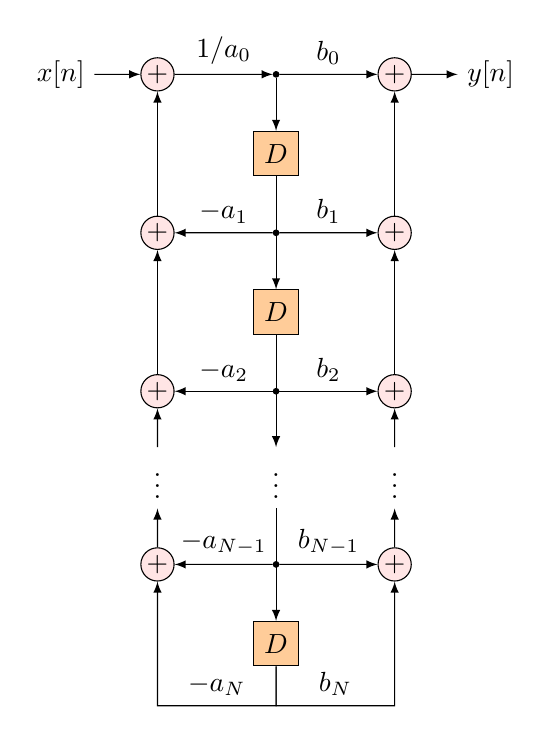
\begin{tikzpicture}
[
	scale=0.8,
	delay/.style={draw=black, fill=orange!40, minimum width=1.6em, minimum height=1.6em},
	adder/.style={circle, draw=black, fill=pink!40, minimum width=1.2em, minimum height=1.2em, inner sep=0},	
	br/.style={circle, draw=black, fill=black, minimum width=0.2em, minimum height=0.2em, inner sep=0},		
]

      \matrix (m) [row sep=5mm, column sep=10mm]{
      \node [adder] (m00) {$+$}; & \node[br] (m01)  {}; & \node [adder] (m03) {$+$}; \\
       &\node [delay] (m11) {$D$}; \\
       \node [adder] (m20) {$+$}; & \node[br] (m21)  {}; & \node [adder] (m23) {$+$}; \\
       &\node [delay] (m31) {$D$};  & \\
       \node [adder] (m40) {$+$}; & \node[br] (m41)  {}; & \node [adder] (m43) {$+$}; \\
        \node [] (m50) {$\vdots$}; & \node [] (m51) {$\vdots$};  & \node [] (m53) {$\vdots$}; \\             
        \node [adder] (m60) {$+$}; & \node[br] (m61)  {}; & \node [adder] (m63) {$+$}; \\
       &\node [delay] (m71) {$D$}; \\       
       \coordinate  (m80) {}; & \coordinate[] (m81)  {}; & \coordinate [] (m83) {};\\     
% 
      };



      \foreach \i/\j in {0/1, 1/3, 3/5, 5/7}
    {
		\draw[-latex] (m\i 1) -- (m\j 1);
			
    }
% 
      \foreach \i/\j in {0/2, 2/4, 4/5, 5/6}
    {
		\draw[latex-] (m\i 0) -- (m\j 0);
		\draw[latex-] (m\i 3) -- (m\j 3);				
    }
% 
% 
   \draw[-latex] (m00) -- node[midway, above] {$1/a_0$} (m01);
    \draw[-latex] (m01) -- node[midway, above] {$b_0$} (m03);
% 
    \draw[latex-] (m20)  -- node[midway, above] {$-a_1$} (m21);
    \draw[-latex] (m21)  -- node[midway, above] {$b_1$} (m23);
    
    \draw[latex-] (m40)  -- node[midway, above] {$-a_2$} (m41);
    \draw[-latex] (m41)  -- node[midway, above] {$b_2$} (m43);
%     
    \draw[latex-] (m60)  -- node[midway, above] {$-a_{N-1}$} (m61);
    \draw[-latex] (m61)  -- node[midway, above] {$b_{N-1}$} (m63);    
% 
	\draw[-latex] (m71) -- (m81) -- node[midway, above] {$b_{N}$} (m83)  -- (m63);
	\draw[latex-] (m60) -- (m80) -- node[midway, above] {$-a_{N}$} (m81)  -- (m71);

	\draw[latex-] (m00) -- ++(-1,0) node[anchor=east] {$x[n]$};
	\draw[-latex] (m03) -- ++(1,0) node[anchor=west] {$y[n]$};

\end{tikzpicture}